\chapter{函数作为无限维向量}
\label{chap:functions-as-vectors}
\label{chap:function-spaces}

拟合一条曲线时，要比较的是两条完整的曲线；研究一列近似函数时，要问这一列整体上是否趋于某个函数。两件事都要求把一个完整的函数当作一个对象，对它做加法、做缩放、量距离。

这种看法可以从一列数开始。把函数$f$在一串输入$x_1,x_2,\ldots$处的取值排起来，就得到一个很长的向量：
\[
 f\ \longleftrightarrow\ [\ldots,a_1,a_2,a_3,\ldots],\qquad a_k=f(x_k).
\]
输入取得越密，这一列就越长。把所有输入都算上时，函数就成了一个“每个输入占一个分量”的向量，下标取遍定义域。本章的标题说的就是这件事。

卷二在有限维线性空间中建立了向量的语言：相加、数乘、基、坐标、范数。本章沿着上面的类比把这些概念逐一搬到函数上，每搬一个都问两个问题：它在函数上的对应物是什么，这个类比又在哪里失效。

第~\ref{sec:fvec-linear-operations}节说明函数的逐点运算正是向量的逐分量运算，由此得到函数空间。第~\ref{sec:fvec-dimension}节比较“定义域有多少点”与“空间有多少维”，这两个数并不相同：定义在整条实轴上、次数不超过$2$的多项式只组成三维空间。维数无限以后，有限线性组合不再够用，第~\ref{sec:fvec-infinite-expansions}节讨论用无穷多项之和表示元素时要回答哪些问题。第~\ref{sec:fvec-closed-ball-noncompact}节处理一个有限维中不会出现的现象：单位球里放得下无穷多个彼此远离的点。

本章只建立线性结构并指出无限维带来的困难。函数之间的范数、完备性及$L^p$空间在第~\ref{chap:function-normed-spaces}章研究；内积、正交投影和正交展开在第~\ref{chap:function-inner-product-spaces}章研究；有界函数类在给定精度下需要多少代表，在第~\ref{chap:function-class-covers}章研究。

\section{函数的线性运算}
\label{sec:fvec-linear-operations}

两条温度曲线可以取平均，一个信号可以整体放大一倍，一个近似函数减去目标函数得到误差函数。这些操作都作用于整个函数，结果仍是一个函数。它们遵守的规则与向量运算完全相同，原因就在于函数可以看成“每个输入占一个分量”的向量。

全章固定标量域$\mathbb K$，它是实数域$\mathbb R$或复数域$\mathbb C$。需要区分时，我们写明“实函数空间”或“复函数空间”；不写明时，结论对两种情形都成立。函数空间的元素是整个函数，按习惯用普通字母$f,g,h$或$x,y$表示，不用粗体。

\paragraph{逐点加法与数乘}
先做一个有限的计算。在$[0,1]$上取$f(x)=x^2$与$g(x)=1-x$，在四个等距点$x_1=0$、$x_2=\tfrac13$、$x_3=\tfrac23$、$x_4=1$处读出取值。每个函数由此变成一个四维向量：
\[
 \begin{aligned}
 [f(x_1),f(x_2),f(x_3),f(x_4)]&=[0,\tfrac19,\tfrac49,1],\\
 [g(x_1),g(x_2),g(x_3),g(x_4)]&=[1,\tfrac23,\tfrac13,0].
 \end{aligned}
\]
把这两个向量逐分量相加，得到
\[
 [1,\tfrac79,\tfrac79,1].
\]

函数$h(x)=x^2-x+1$在这四点的取值恰好是这四个数，而$h$正是在每个$x$处把$f(x)$与$g(x)$加起来的结果。所以“两个采样向量相加”与“两个函数在每个输入处相加”给出同一列数。

这个结论与采样点的个数无关。把四个点换成四十个、四百个，向量变长，每个分量上做的事不变。取遍全部输入时，就得到函数的加法。图~\ref{fig:fvec-pointwise-addition}左边是四维向量的相加，右边是取遍全部输入后的情形：在任何一个$x$处，把蓝色高度与绿色高度首尾相接，就落到$f+g$的曲线上。

\begin{BookInlineFigure}
  \centering
  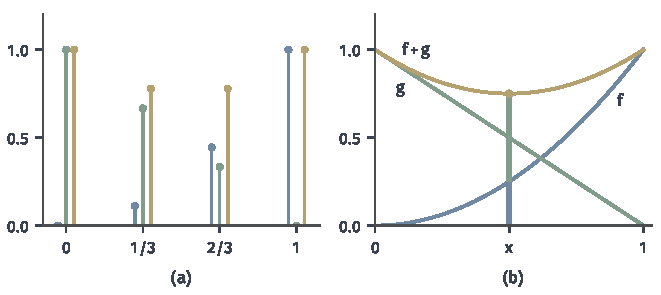
\includegraphics[width=112mm]{figures/04-spaces-measures-and-geometry/03-function-spaces/matplotlib/fvec-pointwise-addition/figure.pdf}
  \caption{函数相加就是逐分量相加。蓝色为$f(x)=x^2$，绿色为$g(x)=1-x$，黄色为二者之和。(a)四个采样点上的取值，每点从左到右依次是$f$、$g$、$f+g$的分量。(b)全部输入上的曲线；在一个固定的$x$处，蓝色线段与绿色线段接起来的总高度等于$f(x)+g(x)$。}
  \label{fig:fvec-pointwise-addition}
\end{BookInlineFigure}

现在写出一般的定义。固定一个非空集合$X$，称为输入集合，考虑全体函数$f:X\to\mathbb K$组成的集合，记为$\mathbb K^X$。这个记号本身就是类比：$\mathbb K^d$的元素给每个下标$k\in\{1,\ldots,d\}$指定一个数，$\mathbb K^X$的元素给每个$x\in X$指定一个数。两个函数的和与一个函数的数乘都在每个输入处分别计算：
\begin{equation}
 (f+g)(x)=f(x)+g(x),\qquad (cf)(x)=c\,f(x),
 \label{eq:fvec-pointwise-operations}
\end{equation}
其中$x\in X$，$c\in\mathbb K$。零元素是处处取零的\term{零函数}（zero function），$f$的负元是$x\mapsto-f(x)$。式~\eqref{eq:fvec-pointwise-operations}称为\term{逐点运算}（pointwise operations）。

逐点运算满足线性空间的八条运算规则，验证方法是把每条规则放到一个固定的输入处检查。以加法交换律为例，要证$f+g=g+f$，而两个函数相等的意思是它们在每个输入处取值相同。任取$x\in X$，由式~\eqref{eq:fvec-pointwise-operations}和数的交换律，
\[
 (f+g)(x)=f(x)+g(x)=g(x)+f(x)=(g+f)(x).
\]

结合律、分配律和零元、负元的规则都这样逐点继承自$\mathbb K$中的运算，所以$\mathbb K^X$在逐点运算下是$\mathbb K$上的线性空间。这与验证$\mathbb K^d$是线性空间时逐分量检查的做法相同。线性空间与子空间的一般定义、基与坐标，可参考\BookChapterRef{chap:linear-representation}{卷二第2章“线性空间、映射与坐标”}。

改变输入集合$X$，就得到熟悉的对象。取$X=\{1,\ldots,d\}$，函数就是$d$维向量。取$X=\mathbb N_+=\{1,2,3,\ldots\}$，一个函数$x:\mathbb N_+\to\mathbb K$就是一个数列$x=(x_1,x_2,\ldots)$，其中$x_k=x(k)$，式~\eqref{eq:fvec-pointwise-operations}这时是逐项相加与逐项数乘。取$X=[0,1]$，就是区间上的函数。图~\ref{fig:fvec-index-to-function}把这三种情形放在一起：横轴都是“下标”，纵轴都是“这个下标上的数”。

\begin{BookInlineFigure}
  \centering
  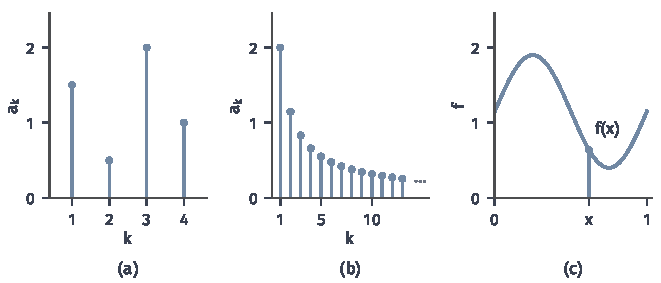
\includegraphics[width=112mm]{figures/04-spaces-measures-and-geometry/03-function-spaces/matplotlib/fvec-index-to-function/figure.pdf}
  \caption{同一种构造的三个例子。(a)$X=\{1,2,3,4\}$时是四维向量。(b)$X=\mathbb N_+$时是数列，下标可以一直延伸下去。(c)$X=[0,1]$时下标连成一片，竖线所示的是下标$x$上的数$f(x)$，竖线的顶点连成了函数的图像。}
  \label{fig:fvec-index-to-function}
\end{BookInlineFigure}

类比在这里出现第一个边界。$X=[0,1]$时，输入有不可数个，无法排成$a_1,a_2,\ldots$这样的一列，所以$[\ldots,f(x),\ldots]$只是一幅图景，不是真的列表。好在式~\eqref{eq:fvec-pointwise-operations}用不着排序，它只要求对每个$x$分别计算。表~\ref{tab:fvec-dictionary}汇总了目前的对应关系。

\begin{BookInlineTable}
  \centering
  \begin{tabular}{@{}ll@{}}
    \toprule
    有限维向量$a\in\mathbb K^d$ & 函数$f\in\mathbb K^X$\\
    \midrule
    下标$k\in\{1,\ldots,d\}$ & 输入$x\in X$\\
    分量$a_k$ & 取值$f(x)$\\
    逐分量相加$a+b$ & 逐点相加$f+g$\\
    逐分量数乘$ca$ & 逐点数乘$cf$\\
    零向量 & 零函数\\
    $a=b$：每个分量相等 & $f=g$：每个输入处取值相等\\
    \bottomrule
  \end{tabular}
  \caption{有限维向量与函数的对应。左右两列的运算规则相同，差别只在下标集合。}
  \label{tab:fvec-dictionary}
\end{BookInlineTable}

\paragraph{线性子空间的核验}
实际使用的通常不是全体函数，而是满足某种要求的函数，例如连续函数或多项式。这就像在$\mathbb R^3$中只看一个过原点的平面。要在这样的集合$V\subseteq\mathbb K^X$中继续使用线性空间的语言，须核对三条：零函数属于$V$；$V$中两个函数之和仍在$V$中；$V$中函数的数乘仍在$V$中。三条都成立时，$V$是$\mathbb K^X$的线性子空间，本身也是线性空间，下面简称为\term{函数空间}（function space）。

几个常用的集合都通过了核验。闭区间上的连续函数全体$C[a,b]$是线性子空间，因为常数零连续，连续函数的和与数乘仍连续。次数不超过$m$的多项式全体$P_m$是线性子空间，因为两个这样的多项式相加不会提高次数。

数列也有同样的例子。收敛到零的数列全体记为$c_0$，它是线性子空间：若$x_k\to0$、$y_k\to0$，则$x_k+y_k\to0$，$cx_k\to0$。只有有限项非零的数列全体记为$c_{00}$，它也是线性子空间，因为两个数列的非零项都只有有限个时，和的非零项也只有有限个。

约束一个分量的取值，能看出子空间与非子空间的区别。集合$\{f\in C[0,1]:f(0)=0\}$把“下标$0$上的分量”固定为零，它是线性子空间，正如$\mathbb R^3$中的平面$x_1=0$。集合$\{f\in C[0,1]:f(0)=1\}$则对应不过原点的平面$x_1=1$：它不含零函数，两个成员相加后在$0$处取$2$，也不封闭。

失败还可以更隐蔽。$\mathbb R^2$中两条坐标轴的并集对数乘封闭，但$(1,0)+(0,1)$已经离开了这个集合。函数空间中也有同样的情形，考虑参数族
\[
 \mathcal R=\{x\mapsto a\max(0,x-t):a,t\in\mathbb R\},
\]
其中每个成员的图像是一条折线，斜率至多改变一次。

取$\mathcal R$中的两个成员$f(x)=\max(0,x)$与$g(x)=\max(0,x-1)$，分段写出它们的和：
\[
 (f+g)(x)=\begin{cases}0,&x\leq0,\\x,&0<x\leq1,\\2x-1,&x>1.\end{cases}
\]
斜率在$x=0$处由$0$变为$1$，在$x=1$处由$1$变为$2$，共改变两次，所以$f+g\notin\mathcal R$。$\mathcal R$对数乘封闭、对加法不封闭，和两条坐标轴的并集属于同一类。这样的族可以作为逼近工具，但不能直接当作线性空间使用。

\paragraph{函数值、函数元素与坐标}
向量有下标$k$、分量$a_k$和整个向量$a$三个层次，函数也一样。输入$x\in X$是一个位置；$f(x)\in\mathbb K$是这个位置上的数；$f$本身是整条对应规则，是函数空间中的一个元素。说“$f=g$”是在比较元素，要求所有位置的值都相同；说“$f(x_0)=g(x_0)$”只比较了一个位置。

坐标是另一回事，它依赖另外选定的基。在$P_2$中取多项式$p(x)=2-x+3x^2$，相对于基$1,x,x^2$，它的坐标是系数$(2,-1,3)$。改用基$1,x-1,(x-1)^2$时，要把$p$按$x-1$重新整理。令$t=x-1$，把$x=t+1$代入$p$，得到
\[
 p=2-(t+1)+3(t+1)^2.
\]
展开平方并合并同类项，得到
\[
 p=4+5t+3t^2.
\]
换回$x$，就是
\[
 p(x)=4+5(x-1)+3(x-1)^2,
\]
所以新的坐标是$(4,5,3)$。

元素$p$没有变，变的是记录它的方式。这与卷二中同一个向量在两组基下有两列坐标是一回事。图~\ref{fig:fvec-two-coordinates}中两张图的蓝色曲线是同一条，只是拆成了不同的三个部分。

\begin{BookInlineFigure}
  \centering
  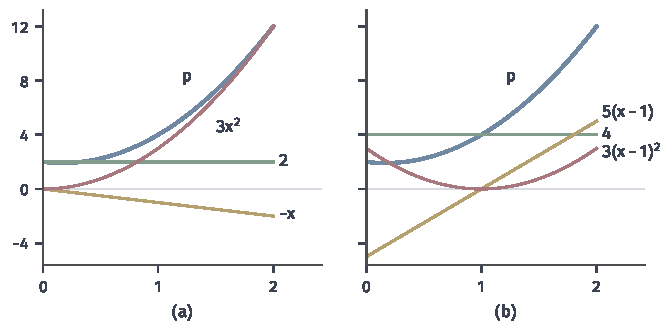
\includegraphics[width=112mm]{figures/04-spaces-measures-and-geometry/03-function-spaces/matplotlib/fvec-two-coordinates/figure.pdf}
  \caption{同一个函数的两种分解。蓝色曲线都是$p(x)=2-x+3x^2$。(a)拆成$2$、$-x$、$3x^2$三部分，坐标为$(2,-1,3)$。(b)拆成$4$、$5(x-1)$、$3(x-1)^2$三部分，坐标为$(4,5,3)$。在每个$x$处，同一张图中三条细线的高度之和等于蓝色曲线的高度。}
  \label{fig:fvec-two-coordinates}
\end{BookInlineFigure}

函数值$p(1)=4$恰好等于第二组坐标的第一项，因为另外两个基函数在$x=1$处都为零。这是这组基的性质，不是坐标的一般含义：第一组坐标的第一项$2$等于$p(0)$，并不等于$p(1)$。

至此，一个函数有了两种“一列数”。一种是取值列，下标是输入$x$，它不需要选基。另一种是系数列，下标是基函数的编号，它随基改变。本章开头的$[\ldots,a_1,a_2,\ldots]$可以按这两种方式来读，下一节会把二者的关系写成矩阵。

\paragraph{乘法与微分不是一般的内部运算}
向量也可以逐分量相乘，但线性空间的定义用不到这种运算。函数同样如此：逐点乘法$(fg)(x)=f(x)g(x)$在某些集合上有意义，却不属于线性结构。$P_m$对乘法不封闭，因为$x^m\in P_m$，而$x^m\cdot x=x^{m+1}\notin P_m$。

求导$f\mapsto f'$也要看空间。$C[0,1]$对乘法封闭，对求导却不封闭：$f(x)=\lvert x-\tfrac12\rvert$连续，但在$\tfrac12$处不可导，$f'$不是$[0,1]$上处处有定义的函数。

所以讨论某个函数空间时，加法与数乘是自带的运算；乘积和导数是另外的操作，要单独说明它们从哪个空间送到哪个空间。例如求导把$P_2$送入$P_2$，而且是线性的。若用基$1,x,x^2$的坐标表示，把$a_0+a_1x+a_2x^2$求导得到$a_1+2a_2x$，这个操作就是一个矩阵：
\[
 \begin{bmatrix}a_1\\2a_2\\0\end{bmatrix}
 =\begin{bmatrix}0&1&0\\0&0&2\\0&0&0\end{bmatrix}
 \begin{bmatrix}a_0\\a_1\\a_2\end{bmatrix}.
\]

把前面的$(2,-1,3)$代入，得到$(-1,6,0)$，也就是$p'(x)=-1+6x$。乘一个固定函数$g$的操作也有这样的矩阵形式：在采样点上，它是对角元为$g(x_1),\ldots,g(x_n)$的对角矩阵。这样的映射在无限维空间中称为线性算子，在第~\ref{chap:linear-operators}章研究；可微性的推广则由第~\ref{chap:smoothing-weak-derivatives}章的弱导数承担。

\section{函数空间的维数}
\label{sec:fvec-dimension}

线性空间的维数是张成整个空间所需的最少方向数，也就是一组基中元素的个数。函数空间的维数同样按这个定义计算。困难在于函数还带着一个输入集合，容易让人把“输入有多少个点”误当成“空间有多少维”。类比$[\ldots,f(x),\ldots]$提示每个输入占一个分量，但下面会看到，只有输入集合有限时，点数才恰好等于$\mathbb K^X$的维数；一般的函数空间只取其中一部分函数，维数可以远小于点数。

\subsection{有限维函数空间}
\label{sec:fvec-finite-dimensional}

最直接的有限维函数空间来自有限的输入集合。设$X=\{x_1,\ldots,x_m\}$有$m$个不同的点。一个函数$f:X\to\mathbb K$由它的$m$个取值$f(x_1),\ldots,f(x_m)$完全确定，所以我们期望$\mathbb K^X$与$\mathbb K^m$是同一个空间的两种写法。

\paragraph{指示函数基}
$\mathbb K^m$的标准基$e_i$在第$i$个分量上取$1$，其余分量取$0$。把这句话照搬到函数上，就是为每个点准备一个只在该点取$1$的函数，即\term{指示函数}（indicator function）
\[
 \delta_i(x)=\begin{cases}1,&x=x_i,\\0,&x\neq x_i,\end{cases}\qquad i=1,\ldots,m.
\]

任意$f\in\mathbb K^X$都可以写成这些函数的组合：
\begin{equation}
 f=\sum_{i=1}^mf(x_i)\,\delta_i.
 \label{eq:fvec-indicator-expansion}
\end{equation}
验证方法是比较两边在每个$x_j$处的取值。右边求和时，只有$i=j$的一项不为零，所以右边在$x_j$处等于$f(x_j)$，与左边相同。于是$\delta_1,\ldots,\delta_m$张成$\mathbb K^X$。

这组函数也线性无关。设$\sum_ic_i\delta_i$是零函数，在$x_j$处取值，得到
\[
 c_j=\sum_{i=1}^mc_i\delta_i(x_j)=0,
\]
这对每个$j$都成立。所以$\delta_1,\ldots,\delta_m$是一组基，$\dim\mathbb K^X=m$。式~\eqref{eq:fvec-indicator-expansion}说明，$f$在这组基下的坐标恰好是它的$m$个取值。

这时函数的线性运算完全变成坐标运算。取$X=\{0,1,2\}$，设$f$与$g$的取值分别是下面两列数：
\[
 f=(1,0,4),\qquad g=(2,-1,1).
\]
式~\eqref{eq:fvec-pointwise-operations}在每点分别计算，于是$2f-g$的取值是
\[
 2f-g=(2\cdot1-2,\ 2\cdot0+1,\ 2\cdot4-1)=(0,1,7).
\]
这三个数也就是$2f-g$的坐标。图~\ref{fig:fvec-indicator-basis}把$f$拆成了三个指示函数的高度，与把$\mathbb K^3$的向量拆成标准基是同一幅图。

\begin{BookInlineFigure}
  \centering
  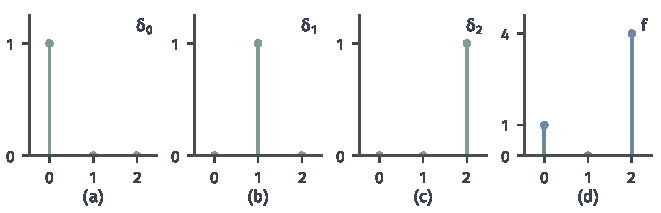
\includegraphics[width=112mm]{figures/04-spaces-measures-and-geometry/03-function-spaces/matplotlib/fvec-indicator-basis/figure.pdf}
  \caption{$X=\{0,1,2\}$上的指示函数基。(a)至(c)是三个基函数$\delta_0,\delta_1,\delta_2$，每个只在一个输入处取$1$。(d)是$f=\delta_0+4\delta_2$，它的三个取值$(1,0,4)$就是坐标。}
  \label{fig:fvec-indicator-basis}
\end{BookInlineFigure}

\paragraph{多项式基与坐标}
有限维函数空间不一定来自有限的输入集合。在整个实轴上考虑$P_m$，即次数不超过$m$的实多项式全体。每个$p\in P_m$可以写成
\[
 p(x)=a_0+a_1x+\cdots+a_mx^m,
\]
所以$1,x,\ldots,x^m$张成$P_m$。

要说明它们是一组基，还须核对线性无关。设$\sum_{k=0}^mc_kx^k$对每个实数$x$都等于零。左边是一个次数不超过$m$的多项式，若系数不全为零，它至多有$m$个根；而它在无穷多个点处取零，所以每个$c_k=0$。于是
\begin{equation}
 \dim P_m=m+1,
 \label{eq:fvec-polynomial-dimension}
\end{equation}
系数$(a_0,\ldots,a_m)$是$p$相对于这组基的坐标。

这个例子把两种“个数”分开了。$P_m$的定义域$\mathbb R$有不可数个点，空间却只有$m+1$维：一旦知道$m+1$个系数，整条曲线在每一点的值都确定了。可以想象一个不可数长的取值列，它的全部分量由$m+1$个数决定。维数只看张成整个空间需要多少方向，与函数定义在多少个点上无关。

在$P_2$上还可以把取值列与系数列的关系算清楚。上一节的$p(x)=2-x+3x^2$，系数列是$(2,-1,3)$。在三个点$0,1,2$处读取值，得到取值列
\[
 p(0)=2,\qquad p(1)=4,\qquad p(2)=12.
\]
一般地，对$a_0+a_1x+a_2x^2$在这三点取值，就是用一个矩阵乘系数列：
\begin{equation}
 \begin{bmatrix}p(0)\\p(1)\\p(2)\end{bmatrix}
 =\begin{bmatrix}1&0&0\\1&1&1\\1&2&4\end{bmatrix}
 \begin{bmatrix}a_0\\a_1\\a_2\end{bmatrix}.
 \label{eq:fvec-vandermonde}
\end{equation}

这个矩阵的行列式等于$(1-0)(2-0)(2-1)=2\neq0$，所以它可逆。这意味着系数列和取值列互相决定，$(2,-1,3)$与$(2,4,12)$只是同一个元素的两列坐标。图~\ref{fig:fvec-coefficient-point}把这三者放在一起：同一条抛物线，在两个坐标系中各是一个点。

\begin{BookInlineFigure}
  \centering
  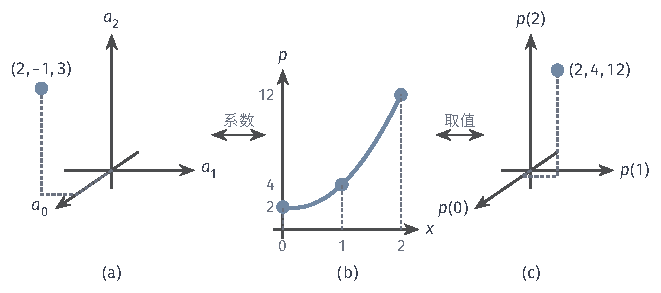
\includegraphics[width=111.919mm]{figures/04-spaces-measures-and-geometry/03-function-spaces/tikz/fvec-coefficient-point/figure.pdf}
  \caption{$P_2$中一个元素的三种面貌。(b)是曲线$p(x)=2-x+3x^2$，蓝点是它在$0,1,2$处的取值。(a)是它的系数列，在以系数为坐标轴的$\mathbb R^3$中是一个点。(c)是它在三点的取值列，在另一个$\mathbb R^3$中也是一个点。两个点由式~\eqref{eq:fvec-vandermonde}的矩阵互相转换。}
  \label{fig:fvec-coefficient-point}
\end{BookInlineFigure}

取值列也可以就是某组基下的坐标，只要选对基。令
\[
 \begin{aligned}
 \ell_0(x)&=\tfrac12(x-1)(x-2),\\
 \ell_1(x)&=-x(x-2),\\
 \ell_2(x)&=\tfrac12x(x-1).
 \end{aligned}
\]
这三个多项式在$0,1,2$上的取值分别是$(1,0,0)$、$(0,1,0)$、$(0,0,1)$，它们在这三点上的行为和指示函数一样。于是
\[
 p=2\ell_0+4\ell_1+12\ell_2.
\]
直接展开右边，得到$(x^2-3x+2)+(-4x^2+8x)+(6x^2-6x)$，合并后正是$2-x+3x^2$。

\subsection{无限维函数空间}
\label{sec:fvec-infinite-dimensional}

有限维向量的长度可以增加：$\mathbb R^1$可以看作$\mathbb R^2$中第二个分量为零的部分，$\mathbb R^2$又可以看作$\mathbb R^3$的一部分，这样一直延续下去。无限维说的是这个过程永远走不到头。若一个线性空间对每个正整数$n$都含有$n$个线性无关的元素，它就不能由任何有限个元素张成，称为\term{无限维}（infinite-dimensional）的。理由是卷二已经证明，由$k$个元素张成的空间中，线性无关的元素至多有$k$个。

\paragraph{全体多项式}
把次数的上限去掉，考虑全体实多项式组成的空间$P=\bigcup_{m\geq0}P_m$。它是线性子空间，因为两个多项式之和仍是多项式。上一小节的论证对每个$m$都成立，$1,x,\ldots,x^m$线性无关，而$m$可以任意大，所以$P$是无限维的。

也可以直接说明任何有限族都张不成$P$。设$q_1,\ldots,q_k$是有限个多项式，其中最高的次数为$d$。它们的任意线性组合次数都不超过$d$，所以$x^{d+1}$不在它们的张成空间中。无论选哪$k$个多项式，总有更高次的多项式落在外面。

\paragraph{全体数列}
数列空间$\mathbb K^{\mathbb N_+}$中，令$e_k$为第$k$项为$1$、其余各项为$0$的数列，称为第$k$个\term{标准单位列}（standard unit sequence），它是$\mathbb K^d$的标准基向量的直接延续。对任意$n$，若$\sum_{k=1}^nc_ke_k$是零数列，读出第$k$项即得$c_k=0$，所以$e_1,\ldots,e_n$线性无关。$n$任意，数列空间是无限维的。

同样的论证说明，只要输入集合$X$有无穷多个点，不同点的指示函数就构成任意多个线性无关的元素，$\mathbb K^X$都是无限维的。这里类比又碰到一个边界：$X$无限时，式~\eqref{eq:fvec-indicator-expansion}不能原样推广。指示函数的有限组合只在有限个点上不为零，所以常数函数$1$不在它们的张成空间中。取值仍然是每个输入上的数，却不再是一组基下的有限坐标。

\paragraph{每个元素有限与整体无限}
无限维并不意味着每个元素都“需要无穷多个方向”。$P$中的每个多项式只用到有限个单项式，它的系数列$[a_0,a_1,\ldots,a_d,0,0,\ldots]$从某一项起全为零；$c_{00}$中的每个数列也只是有限个$e_k$的组合。无限维说的是整个空间：没有一组固定的有限个方向，能同时表示所有元素。

图~\ref{fig:fvec-finite-support-grid}的前三行是三个多项式的系数列，每一行都只占有限个格子，但占到的最靠右的位置没有统一的上限。第四行不同：$e^x$的系数$1/k!$永远不为零。它不是多项式，因为任何多项式求导足够多次后变为零，而$e^x$求导后不变。

\begin{BookInlineFigure}
  \centering
  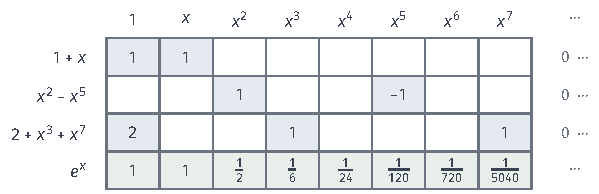
\includegraphics[width=101.469mm]{figures/04-spaces-measures-and-geometry/03-function-spaces/tikz/fvec-finite-support-grid/figure.pdf}
  \caption{系数列的两种形态。每一列对应一个单项式，蓝格是非零系数。前三行是多项式，只占有限个格子，其后全为零，所占范围随元素变化。第四行绿色的$e^x$每一格都不为零，有限个单项式的组合表示不了它。}
  \label{fig:fvec-finite-support-grid}
\end{BookInlineFigure}

数列空间中的常数列$(1,1,\ldots)$与$e^x$处境相同，它不是有限个$e_k$的组合。若想用$e_1,e_2,\ldots$表示这样的元素，就只能借助无穷多项之和，这需要先说明无穷和是什么意思。

\section{无限展开}
\label{sec:fvec-infinite-expansions}

有限维空间中，选定基以后，每个向量都由有限次加法和数乘精确地表示出来，坐标唯一，不涉及任何极限。进入无限维后，这一步分裂成两个问题：有限线性组合到底能覆盖哪些元素；对覆盖不到的元素，无穷多项的部分和能否趋于它，在什么意义下趋于它。数列的结构最简单，本节用数列把这两个问题分开研究，函数的正交展开要用到内积，在第~\ref{chap:function-inner-product-spaces}章讨论。

\subsection{代数基与级数表示}
\label{sec:fvec-algebraic-basis-series}

线性代数中的基只允许有限线性组合。把这一要求原样用于无限维空间，就得到下面的定义。

\begin{definition}[代数基]
\label{def:fvec-algebraic-basis}
设$V$是线性空间，$B\subseteq V$。若$B$中任意有限个不同元素线性无关，并且$V$的每个元素都是$B$中有限个元素的线性组合，称$B$为$V$的\term{代数基}（algebraic basis），也称\term{Hamel基}（Hamel basis）。
\end{definition}

定义中的两个条件各管一件事。线性无关保证表示唯一：若同一元素有两种有限表示，相减得到一个等于零的有限组合，各系数之差只能为零。“有限组合”则规定了允许的表示方式：不涉及任何极限，因此不需要事先给空间配上距离。

\paragraph{有限支撑数列与全体数列}
在$c_{00}$中，标准单位列$\{e_k\}_{k\geq1}$是代数基。线性无关上一节已经验证。若$x\in c_{00}$的非零项都在前$n$项之中，则
\[
 x=\sum_{k=1}^nx_ke_k
\]
是一个有限组合，所以$c_{00}$的每个元素都由$\{e_k\}$精确表示，坐标就是数列的各项。全体多项式$P$的情形相同：把多项式对应到它的系数列，$P$就成了换了名字的$c_{00}$，单项式$x^k$对应$e_{k+1}$。

同一族$\{e_k\}$在全体数列空间$\mathbb K^{\mathbb N_+}$中仍然线性无关，却不再张成整个空间。$e_1,\ldots,e_n$的任何组合从第$n+1$项起全为零，所以常数列$(1,1,\ldots)$不是有限个$e_k$的组合。$\{e_k\}$在$\mathbb K^{\mathbb N_+}$中只是一个线性无关族，它的有限组合恰好覆盖了$c_{00}$。

一般的无限维空间也有代数基，而且任何线性无关族都能扩充为一组代数基。证明要用到选择公理，具体通过Zorn引理进行，篇幅较长，读者可查阅线性代数或集合论的教材。这种存在性证明不给出具体的基，$\mathbb K^{\mathbb N_+}$的代数基至今没有可以写下来的公式。代数基仍然只允许有限组合，因此也不能用它谈论无穷和。

\paragraph{级数表示需要另外核对的内容}
要用$\{e_k\}$表示常数列这样的元素，自然想到写成无穷和$\sum_{k\geq1}x_ke_k$，把它理解为部分和
\[
 s_N=\sum_{k=1}^Nx_ke_k=(x_1,\ldots,x_N,0,0,\ldots)
\]
在$N\to\infty$时的极限。线性空间本身不提供极限，所以写下这个级数之前，先要规定“部分和趋于某个元素”的含义。

规定好收敛的意义之后，还要分别核对三件事。其一是收敛性：对给定的系数，部分和是否收敛。其二是表示范围：能够这样写出的元素是否覆盖整个空间。其三是唯一性：同一个元素能否有两组不同的系数。有限维时三者都自动成立，无限维时它们都依赖所选的收敛意义，需要逐项证明。

唯一性的失败最出乎意料，因为有限维中线性无关足以保证唯一。下面的例子采用逐项收敛的意义：对每个固定的$j$，第$j$项收敛。在数列空间中令
\[
 u_0=e_1,\qquad u_k=e_k-e_{k+1},\quad k\geq1.
\]

这族元素的任意有限个线性无关。设$a_0u_0+\sum_{k=1}^na_ku_k$是零数列。读第$n+1$项得$-a_n=0$；再依次读第$n$项、第$n-1$项直到第$2$项，由$a_k-a_{k-1}=0$得到$a_{n-1}=\cdots=a_1=0$；最后读第$1$项，得$a_0=0$。

然而$e_1$有两种展开。第一种就是$e_1=u_0$，系数列为$(1,0,0,\ldots)$。第二种来自逐项相消：前$N$个$u_k$之和是
\[
 \sum_{k=1}^Nu_k=e_1-e_{N+1},
\]
当$N\geq j$时，它的第$j$项等于$e_1$的第$j$项，所以逐项收敛到$e_1$，系数列为$(0,1,1,\ldots)$。在有限组合的意义下这族元素线性无关，在无穷和的意义下却有两种展开。

也不能默认每个无限维空间都有一族可数元素，使每个元素都能写成它们的级数。考虑有界数列，以两个数列各项之差的上确界衡量它们的距离。对$\mathbb N_+$的每个子集$S$，令$\chi_S$在$k\in S$处取$1$、其余取$0$。两个不同子集给出的数列在某一项相差$1$，所以彼此距离为$1$，这样的数列有不可数个。

假设某个可数族$\{u_j\}$能把每个有界数列都写成在这种距离下收敛的级数$\sum_ja_ju_j$。那么系数取有理数（复情形取实部、虚部都为有理数）的有限组合就构成一个可数集，并且能以任意精度逼近每个有界数列：先截断级数，再把系数换成相近的有理数。

于是以每个$\chi_S$为中心、半径$\tfrac12$的开球中都要有这个可数集的点。这些球两两不交，不可数个球却只分到可数个点，矛盾。具有可数稠密子集的空间称为可分空间，其一般定义见第~\ref{chap:topological-spaces}章。可数级数表示的存在，要求空间可分。

\subsection{展开的收敛}
\label{sec:fvec-expansion-convergence}

向量列有两种自然的“接近”方式。一种逐项比较：对每个固定的分量，误差都趋于零，称为逐项收敛。另一种统一比较：所有分量上误差的最大值趋于零。在$\mathbb K^d$中两者没有区别。设每个分量的误差都趋于零，给定$\varepsilon>0$，第$k$个分量从第$N_k$步起误差小于$\varepsilon$。取
\[
 N=\max\{N_1,\ldots,N_d\},
\]
从第$N$步起，全部$d$个分量同时误差小于$\varepsilon$。

这一步用到分量只有有限个，有限个数才一定有最大值。分量无穷多时，$N_k$可能没有上界，每个分量迟早对上，却没有一个共同的时刻。下面用两个数列的截断说明，这两种意义给出的结论可以不同。

\paragraph{常数列的截断}
取$x=(1,1,1,\ldots)$，部分和$s_N=(1,\ldots,1,0,0,\ldots)$保留前$N$项、其余置零。误差$x-s_N$的前$N$项为$0$，从第$N+1$项起全为$1$。

固定任意一项$k$，只要$N\geq k$，第$k$项的误差就是$0$，所以$s_N$逐项收敛到$x$。但所有项上误差的最大值是
\[
 \sup_{k\geq1}\lvert x_k-(s_N)_k\rvert=1,\qquad N=1,2,\ldots,
\]
不随$N$减小。每一项迟早都对，可“尚未对上的项”永远存在，只是向后移动。

\paragraph{调和数列的截断}
再取$y=(1,\tfrac12,\tfrac13,\ldots)$，作同样的截断$t_N=(1,\ldots,\tfrac1N,0,\ldots)$，逐项收敛同样成立。误差$y-t_N$的非零项是$\tfrac1{N+1},\tfrac1{N+2},\ldots$，其中最大的是第一项，所以
\begin{equation}
 \sup_{k\geq1}\lvert y_k-(t_N)_k\rvert=\frac1{N+1}\to0.
 \label{eq:fvec-harmonic-truncation}
\end{equation}
这里统一的误差也趋于零：尾部的各项本身在变小，截掉它们造成的误差随之变小。图~\ref{fig:fvec-truncation-error}并排画出了这两次截断。

\begin{BookInlineFigure}
  \centering
  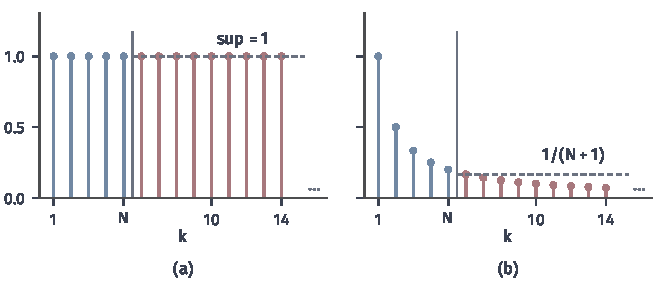
\includegraphics[width=112mm]{figures/04-spaces-measures-and-geometry/03-function-spaces/matplotlib/fvec-truncation-error/figure.pdf}
  \caption{同样的截断，不同的尾部。这里$N=5$，竖线左侧蓝色为保留的项，右侧红色为截掉的项，也就是误差，虚线标出误差的上确界。(a)常数列的尾部一直保持高度$1$，$N$增大时只是整体右移。(b)调和数列的尾部越来越低，上确界为$1/(N+1)$，随$N$增大而趋于零。}
  \label{fig:fvec-truncation-error}
\end{BookInlineFigure}

\paragraph{收敛意义的选择}
两个级数形式完全相同，都是$\sum_kx_ke_k$，区别只在系数。表~\ref{tab:fvec-truncation-compare}对比了两种误差给出的结论。在逐项收敛的意义下，每个数列都能这样展开；在统一误差的意义下，只有尾部趋于零的数列才能这样展开，也就是恰好$c_0$中的数列。所以“级数收敛”本身不是一个完整的陈述，必须说明用哪种误差衡量。

\begin{BookInlineTable}
  \centering
  \begin{tabular}{@{}lll@{}}
    \toprule
    误差的衡量方式 & $x=(1,1,1,\ldots)$ & $y=(1,\tfrac12,\tfrac13,\ldots)$\\
    \midrule
    逐项 & 收敛 & 收敛\\
    所有项的上确界 & 恒等于$1$，不收敛 & $1/(N+1)$，收敛\\
    \bottomrule
  \end{tabular}
  \caption{同一种截断在两种误差下的结论。}
  \label{tab:fvec-truncation-compare}
\end{BookInlineTable}

函数的情形相同，系数列$[1,1,\tfrac12,\tfrac16,\ldots]$就是一个例子。$e^x$的部分和是
\[
 s_N(x)=\sum_{k=0}^N\frac{x^k}{k!}.
\]
先在$[0,1]$上看误差。对$0\leq x\leq1$，把每个$x^k$放大到$1$，得到
\[
 0\leq e^x-s_N(x)=\sum_{k\geq N+1}\frac{x^k}{k!}\leq\sum_{k\geq N+1}\frac1{k!}.
\]

右边从$k=N+1$起，每一项不超过前一项的一半，所以用等比级数控制它：
\begin{equation}
 \sup_{0\leq x\leq1}\lvert e^x-s_N(x)\rvert\leq\frac{2}{(N+1)!}.
 \label{eq:fvec-exp-truncation}
\end{equation}
取$N=3$时，这个上界是$\tfrac1{12}$。所以在$[0,1]$上，统一误差趋于零。

换到整条实轴，结论就变了。在每个固定的$x$处，$s_N(x)$仍趋于$e^x$，因为这个幂级数处处收敛。但固定$N$后，对$x>0$有
\[
 e^x-s_N(x)\geq\frac{x^{N+1}}{(N+1)!},
\]
右边随$x\to+\infty$趋于无穷。所以每个$N$的统一误差都是无穷大，同一个级数在$\mathbb R$上逐点收敛、不一致收敛。

对一列近似函数，可以要求每个输入处的值收敛（逐点收敛），可以要求所有输入上的最大误差趋于零（一致收敛），也可以要求误差的积分趋于零。这三种意义互不等价。第~\ref{chap:function-normed-spaces}章用范数统一表达整体误差并比较这些收敛方式，具体表示及其截断误差则在第~\ref{chap:function-inner-product-spaces}章的正交展开和第~\ref{chap:function-approximation}章的函数逼近中研究。

\section{无限维闭球不紧}
\label{sec:fvec-closed-ball-noncompact}

在$\mathbb R^d$中，有界序列总有收敛子列，闭有界集上的连续函数总取到最小值。许多存在性论证都是这样进行的：先找一列越来越好的近似，再从中抽出收敛子列，最后说明极限就是所求的对象。本节说明，这条路在无限维空间中会断。

标准单位列已经显示了问题所在。在$c_0$中用各项之差的上确界作距离，$e_m$与$e_n$（$m\neq n$）在第$m$项相差$1$，其余各项相差不超过$1$，所以二者的距离恰为$1$。这些点都在以零数列为中心、半径为$1$的闭球里，它们彼此隔开，没有任何子列收敛。

本节要证明这不是$c_0$的特殊现象，而是所有无限维赋范空间的共同性质。这里需要用距离衡量“彼此隔开”，所以先回顾卷二的范数。线性空间$V$上的范数$\lVert\cdot\rVert$是满足正定性、齐次性$\lVert cx\rVert=\lvert c\rvert\lVert x\rVert$与三角不等式的非负函数，它诱导距离$d(x,y)=\lVert x-y\rVert$；配有范数的空间称为赋范空间。

有限维情形的范数理论可参考\BookChapterRef{chap:normed-spaces}{卷二第3章“赋范空间”}，无限维的系统讨论在第~\ref{chap:function-normed-spaces}章。本节只用这些公理和距离的语言。

\paragraph{有限维子空间是闭集}
下面的构造要用到这样一个事实：在任意赋范空间中，有限维子空间是闭集。平面上过原点的直线、三维空间中过原点的平面都是闭集，无限维的环境空间里这一点仍然成立。

\begin{lemma}[有限维子空间闭性]
\label{lem:fvec-finite-subspace-closed}
设$X$是赋范空间，$Y\subseteq X$是有限维线性子空间。则$Y$是$X$中的闭集。
\end{lemma}

\begin{proof}
设$y_n\in Y$且在$X$中$y_n\to x$，要证$x\in Y$。收敛序列是柯西列，所以$\{y_n\}$是$Y$中的柯西列。

把$X$的范数限制在$Y$上，$Y$成为一个有限维赋范空间。卷二证明了有限维赋范空间在任意范数下都完备，所以$\{y_n\}$在$Y$中收敛到某个$y$。

这个$y$也是$\{y_n\}$在$X$中的极限。第~\ref{chap:metric-spaces}章说明度量空间中的极限唯一，所以$x=y\in Y$。
\end{proof}

这个论证没有要求$X$完备，只用到$Y$自身的完备性。由闭性，若$x_0\notin Y$，则$x_0$到$Y$的距离
\[
 d(x_0,Y)=\inf_{y\in Y}\lVert x_0-y\rVert
\]
严格为正：否则可在$Y$中取一列$y_n$使$\lVert x_0-y_n\rVert\to0$，闭性给出$x_0\in Y$，矛盾。

\paragraph{Riesz引理}
要在无限维空间中造出彼此远离的单位向量，先看$\mathbb R^2$中是怎样做的。取一条过原点的直线$Y$和线外一点$x_0$，从$x_0$向$Y$作垂线，垂足是$Y$上离$x_0$最近的点。$x_0$减去垂足再归一化，就得到与$Y$垂直的单位向量，它到$Y$的距离恰为$1$。

一般赋范空间没有垂直，$Y$上的最近点也可能不存在，所以要退一步：不取最近点，而取一个几乎最近的点$y_0$。图~\ref{fig:fvec-riesz-lemma}画出了这个做法。$x_0-y_0$不再与$Y$垂直，归一化后的向量$x$略微倾斜，但它到$Y$的距离仍接近$1$。

\begin{BookInlineFigure}
  \centering
  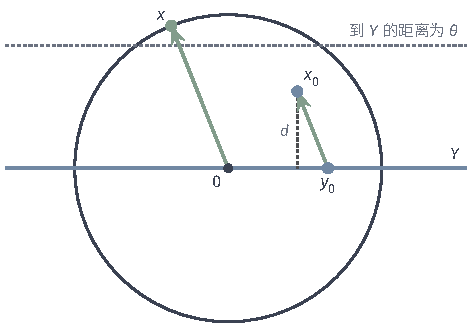
\includegraphics[width=79.904mm]{figures/04-spaces-measures-and-geometry/03-function-spaces/tikz/fvec-riesz-lemma/figure.pdf}
  \caption{Riesz引理的构造在$\mathbb R^2$中的样子。蓝色直线是子空间$Y$，圆是单位球面。$x_0$到$Y$的距离为$d$，$y_0$是$Y$上一个几乎最近的点。把向量$x_0-y_0$（绿色）平移到原点并归一化，得到单位向量$x$，它落在虚线上方，到$Y$的距离不小于$\theta$。}
  \label{fig:fvec-riesz-lemma}
\end{BookInlineFigure}

把这个几何过程写成不等式，就得到下面的引理。

\begin{lemma}[Riesz引理]
\label{lem:fvec-riesz}
设$X$是赋范空间，$Y\subsetneq X$是闭线性子空间，$0<\theta<1$。则存在$x\in X$，使$\lVert x\rVert=1$，并且
\begin{equation}
 \lVert x-y\rVert\geq\theta,\qquad y\in Y.
 \label{eq:fvec-riesz}
\end{equation}
\end{lemma}

\begin{proof}
取$x_0\in X\setminus Y$，记$d=d(x_0,Y)$。由$Y$闭，$d>0$。因为$d/\theta>d$，由下确界的定义可以取$y_0\in Y$使
\[
 d\leq\lVert x_0-y_0\rVert\leq\frac{d}{\theta}.
\]
令$c=\lVert x_0-y_0\rVert$，并取$x=(x_0-y_0)/c$，则$\lVert x\rVert=1$。

对任意$y\in Y$，把$x-y$通分，写成
\[
 x-y=\frac{x_0-(y_0+cy)}{c}.
\]
括号里的$y_0+cy$仍属于线性子空间$Y$，所以分子的范数至少是$d$。于是
\[
 \lVert x-y\rVert\geq\frac{d}{c}\geq\frac{d}{d/\theta}=\theta.
\]
\end{proof}

引理的两个条件都不能去掉。先看“$Y$闭”。在$c_0$中取$Y=c_{00}$，它是真子空间，但不闭。对任意$x\in c_0$，截断$s_N$属于$Y$，并且
\[
 \sup_{k\geq1}\lvert x_k-(s_N)_k\rvert=\sup_{k>N}\lvert x_k\rvert\to0,
\]
所以每个$x$到$Y$的距离都是$0$，式~\eqref{eq:fvec-riesz}对任何$\theta>0$都不成立。

再看$\theta<1$。在有限维中$\theta=1$可以取到，因为最近点存在；无限维中最近点可能取不到，$\theta=1$就可能失败。下面是一个能手算的例子。

\begin{example}[$\theta=1$可能失败]
\label{ex:fvec-riesz-theta-one}
令$X=\{f\in C[0,1]:f(0)=0\}$，范数取$\lVert f\rVert=\max_t\lvert f(t)\rvert$，令
\[
 Y=\Bigl\{f\in X:\int_0^1f(t)\,dt=0\Bigr\}.
\]
$Y$是闭子空间，因为$\lvert\int f-\int g\rvert\leq\lVert f-g\rVert$，积分为零的性质在一致极限下保持。

任取$X$中的单位向量$x$，构造$Y$中逼近它的元素。令$h_n(t)=\min(nt,1)$，则$h_n\in X$，$\lVert h_n\rVert=1$，并且积分为
\[
 \int_0^1h_n(t)\,dt=1-\frac1{2n}.
\]
记$I=\int_0^1x(t)\,dt$，令
\[
 y_n=x-\frac{I}{1-\frac1{2n}}h_n,
\]
它的积分为$I-I=0$，所以$y_n\in Y$。

$x$到$y_n$的距离由$h_n$的系数给出：
\[
 \lVert x-y_n\rVert=\frac{\lvert I\rvert}{1-\frac1{2n}}.
\]
令$n\to\infty$，得到$d(x,Y)\leq\lvert I\rvert$。而$x$连续且$x(0)=0$，所以在$0$附近$\lvert x\rvert<\tfrac12$，又处处有$\lvert x\rvert\leq1$，于是$\lvert I\rvert<1$。

所以$X$中每个单位向量到$Y$的距离都严格小于$1$，$\theta=1$的结论不成立。
\end{example}

\paragraph{两两远离的单位向量}
现在设$X$是无限维赋范空间，用Riesz引理逐个构造单位向量。任取一个单位向量$e_1$。设已经得到单位向量$e_1,\ldots,e_n$，令
\[
 Y_n=\operatorname{span}\{e_1,\ldots,e_n\}.
\]
$Y_n$是有限维子空间，由引理~\ref{lem:fvec-finite-subspace-closed}是闭集；$X$无限维，所以$Y_n\neq X$。对$Y_n$与$\theta=\tfrac12$应用引理~\ref{lem:fvec-riesz}，得到单位向量$e_{n+1}$，它到$Y_n$中每一点的距离都至少为$\tfrac12$。

这样得到的序列$\{e_n\}$有两条性质。其一，它线性无关：$e_{n+1}$到$Y_n$的距离为正，所以$e_{n+1}\notin Y_n$，每个新元素都不能由之前的元素线性表示。其二，它两两远离：对$m<n$，$e_m\in Y_{n-1}$，所以
\begin{equation}
 \lVert e_n-e_m\rVert\geq\frac12,\qquad m\neq n.
 \label{eq:fvec-separated-sequence}
\end{equation}
第~\ref{chap:function-normed-spaces}章构造不等价范数时，还会用到这里的单位列$\{e_n\}$。

有了这列向量，闭球不紧的结论就只差一步。

\begin{theorem}[无限维闭球不紧]
\label{thm:fvec-closed-ball-noncompact}
设$X$是无限维赋范空间。则闭单位球$\bar B=\{x\in X:\lVert x\rVert\leq1\}$不是全有界的，从而不紧。更一般地，对任意$a\in X$与$r>0$，闭球$\{x:\lVert x-a\rVert\leq r\}$都不紧。
\end{theorem}

\begin{proof}
全有界要求对每个$\varepsilon>0$，$\bar B$都能被有限个半径为$\varepsilon$的开球覆盖。取$\varepsilon=\tfrac14$。半径$\tfrac14$的开球中任意两点的距离小于$\tfrac12$，由式~\eqref{eq:fvec-separated-sequence}，每个这样的球至多含有一个$e_n$。$\bar B$中有无穷多个$e_n$，有限个球盖不住它们，所以$\bar B$不全有界。第~\ref{chap:metric-spaces}章证明了紧度量空间必定全有界，故$\bar B$不紧。

也可以直接从序列看：$\{e_n\}$的任何子列都满足式~\eqref{eq:fvec-separated-sequence}，不是柯西列，因而不收敛。

对一般的闭球，映射$x\mapsto a+rx$把$\bar B$一一地映成该闭球，并把距离乘以$r$。若该闭球紧，则$a+re_n$有收敛子列，相应的$e_n$子列也收敛，矛盾。
\end{proof}

证明从头到尾没有用到$X$的完备性。不紧的原因不是“缺少极限点”，而是有界的区域里装得下无穷多个互相隔开的点。

有限维中这样的点只能有有限个，用体积就能数出来。设$\mathbb R^d$的单位球中有$N$个点两两距离至少为$\tfrac12$。以这些点为中心、半径$\tfrac14$的开球两两不交，并且都含在半径$\tfrac54$的球内。比较体积，得到
\[
 N\Bigl(\frac14\Bigr)^d\leq\Bigl(\frac54\Bigr)^d.
\]
约去公因子，就是
\begin{equation}
 N\leq5^d.
 \label{eq:fvec-packing-bound}
\end{equation}
所以$\mathbb R^2$的单位圆盘中至多有$25$个这样的点。这个上界随$d$增大而迅速增大，$d$无限时不再有任何上界，这就是无限维中闭球不紧的直观原因。图~\ref{fig:fvec-bounded-noncompact}(a)是$d=2$的情形。

\paragraph{连续函数的例子}
Riesz引理给出的是存在性。在具体的函数空间中，往往可以直接写出没有收敛子列的有界序列。考虑$C[0,1]$，以两个函数之差的最大绝对值
\[
 d(f,g)=\max_{x\in[0,1]}\lvert f(x)-g(x)\rvert
\]
为距离。连续函数在闭区间上取到最大值，所以$d$有定义；它来自范数$\max_x\lvert f(x)\rvert$，按这一距离收敛就是一致收敛。

\begin{BookInlineFigure}
  \centering
  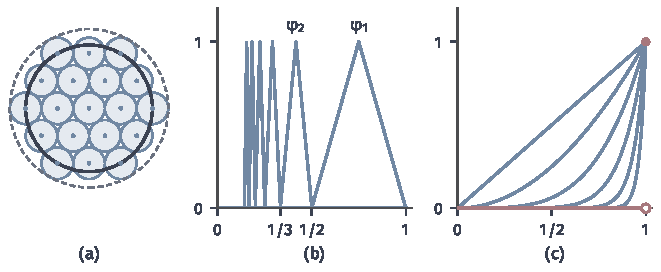
\includegraphics[width=112mm]{figures/04-spaces-measures-and-geometry/03-function-spaces/matplotlib/fvec-bounded-noncompact/figure.pdf}
  \caption{有界而不紧。(a)$\mathbb R^2$单位圆盘（实线）内的$19$个点，两两距离不小于$\tfrac12$，半径$\tfrac14$的小圆盘互不重叠，全部落在半径$\tfrac54$的虚线圆内。(b)在$C[0,1]$中，前六个鼓包$\varphi_n$的支撑互不重叠，高度都是$1$。(c)蓝色为$x^n$（$n=1,2,4,8,16,32$），红色为逐点极限：$[0,1)$上为$0$，在$1$处取$1$。}
  \label{fig:fvec-bounded-noncompact}
\end{BookInlineFigure}

最接近标准单位列的是一列鼓包。对$n\geq1$，令$\varphi_n$在区间$[\tfrac1{n+1},\tfrac1n]$的中点取$1$，在区间两端取$0$，在区间上线性插值，在区间外恒为$0$。图~\ref{fig:fvec-bounded-noncompact}(b)显示，这些鼓包各占一段位置，相当于各占一个“坐标”。

当$m\neq n$时，$\varphi_m$与$\varphi_n$的支撑至多在一点相接，而两函数在该点都为零，所以每点至多有一个函数非零。在$\varphi_n$的峰值点，差的绝对值为$1$，于是
\[
 d(\varphi_m,\varphi_n)=1,\qquad m\neq n.
\]
它们都在以零函数为中心、半径为$1$的闭球内，没有任何子列收敛。

再看$f_n(x)=x^n$，它的表现不同。每个$f_n$满足$0\leq x^n\leq1$，所以也都在同一个闭球内。相邻两项的差$x^n(1-x)$在$x=\tfrac n{n+1}$处取最大值，由此
\[
 d(f_n,f_{n+1})=\Bigl(\frac n{n+1}\Bigr)^n\frac1{n+1}\leq\frac1{n+1},
\]
相邻两项越来越近。序列看上去在收敛，但它仍然没有任何按$d$收敛的子列。

设子列$f_{n_k}$按$d$收敛到某个$g\in C[0,1]$。一致收敛推出逐点收敛，所以对每个$x$，$g(x)=\lim_kx^{n_k}$。当$0\leq x<1$时这个极限是$0$，当$x=1$时是$1$。于是$g$在$[0,1)$上恒为$0$而$g(1)=1$，在$1$处不连续，与$g\in C[0,1]$矛盾。

两个例子失败的方式不同。鼓包的逐点极限是零函数，它就在$C[0,1]$中，可是每个鼓包离它的距离总是$1$，逐点接近不等于一致接近。$x^n$的逐点极限跑出了$C[0,1]$，候选极限根本不在空间里。函数类在什么附加条件下恢复紧性，例如要求一致有界并且等度连续，是第~\ref{chap:metric-space-maps}章和第~\ref{chap:function-class-covers}章的内容。

\section{本章小结}
\label{sec:fvec-summary}

本章开头的问题是：把函数看作向量$[\ldots,f(x),\ldots]$时，有限维线性代数的语言保留了什么，又在哪里失效。表~\ref{tab:fvec-summary}按本章的顺序汇总了答案。

\begin{BookInlineTable}
  \centering
  \begin{tabular}{@{}p{18mm}p{36mm}p{48mm}@{}}
    \toprule
    概念 & 有限维向量 & 无限维函数空间\\
    \midrule
    线性运算 & 逐分量计算 & 逐点计算，规则相同\\
    维数 & 分量个数 & 与输入点数无关，要看函数集合\\
    取值与坐标 & 标准基下坐标就是分量 & 取值一般不是有限组合的坐标\\
    基 & 有限个，有限组合表示全部 & 代数基只允许有限组合，通常写不出\\
    无穷和 & 用不到 & 收敛、范围、唯一性都依赖误差\\
    逐分量与统一误差 & 两种收敛等价 & 两种收敛不同\\
    有界序列 & 总有收敛子列 & 可以没有收敛子列\\
    \bottomrule
  \end{tabular}
  \caption{有限维向量的语言在无限维函数空间中的保留与失效。}
  \label{tab:fvec-summary}
\end{BookInlineTable}

线性运算的部分完整地保留下来。逐点加法与数乘使全体函数$X\to\mathbb K$成为线性空间，数列与有限维向量都是它的特例。连续函数、限次多项式、收敛到零的数列和有限支撑数列都通过了子空间核验。函数作为元素、它在某点的值、它相对于某组基的坐标是三样不同的东西；乘法和求导也不是每个函数空间自带的运算。

维数仍按张成整个空间需要多少方向来计算，与定义域的点数无关。有限输入集合上的函数以指示函数为基，坐标就是函数值。$P_m$定义在整条实轴上，却只有$m+1$维，取值列与系数列由一个可逆矩阵互相决定。全体多项式、全体数列含有任意多个线性无关的元素，因而是无限维的。其中每个元素可能只用到有限个方向，但没有一组固定的有限方向能表示所有元素。

无限维带来两个困难。其一，代数基只允许有限组合，要表示常数列或$e^x$这样的元素就须借助级数，而级数是否收敛、能表示哪些元素、系数是否唯一，都取决于选用的误差。其二，任何无限维赋范空间中，Riesz引理都给出两两距离至少$\tfrac12$的单位向量列，所以正半径闭球都不紧，这一结论不需要空间完备。

这两个困难分别指向后面两章。第~\ref{chap:function-normed-spaces}章用范数规定整体误差，比较不同范数下的收敛，并用完备性保证柯西列的极限留在空间内；第~\ref{chap:function-inner-product-spaces}章再加入内积，用正交投影和正交展开给出收敛的无限表示。闭球不紧则提醒我们：在无限维中求极值或抽收敛子列，需要额外的紧性条件或更弱的收敛概念。

